\section{Geometry of surfaces in $\mathbb R^3$}

\subsection{First fundamental form}
Let $\gamma \colon (a,b) \to \mathbb R^3$ be smooth.
The \vocab{length} of $\gamma$ is
\begin{align*}
	L(\gamma) = \int_a^b \norm{\gamma'(t)} \dd{t}
\end{align*}
This result is independent of the choice of parametrisation.
Let $s \colon (A,B) \to (a,b)$ be a monotonically increasing function, let $\tau(t) = \gamma(s(t))$ and $s \geq 0$.
Then
\begin{align*}
	L(\tau) = \int_A^B \norm{\tau'(t)} \dd{t} = \int_A^B \norm{\gamma'(s(t))} \abs{s'(t)} \dd{t} = \int_a^b \norm{\gamma'(t')} \dd{s} = L(\gamma)
\end{align*}

\begin{lemma}
	If $\gamma \colon (a,b) \to \mathbb R^3$ is continuously differentiable and $\gamma'(t) \neq 0$, then $\gamma$ can be parametrised by arc length, i.e. a parameter s.t. $\norm{\gamma'(s)} = 1 \forall \; s$.
\end{lemma}

\begin{proof}
	Left as an exercise.
\end{proof} 

Let $\Sigma$ be a smooth surface in $\mathbb R^3$, and let $\sigma \colon V \to U \subset \Sigma$ be an allowable parametrisation.
If $\gamma \colon (a,b) \to U$ is smooth, then there exist functions $(u(t), v(t)) \colon (a,b) \to V$ smooth s.t. $\gamma(t) = \sigma(u(t), v(t))$.
Hence $\gamma'(t) = \sigma_u u'(t) + \sigma_v v'(t)$, giving
\begin{align*}
	\norm{\gamma'(t)}^2 = E u'(t)^2 + 2F u'(t) v'(t) + G v'(t)^2
\end{align*}
for functions
\begin{align*}
	E = \inner{\sigma_u, \sigma_u};\quad F = \inner{\sigma_u, \sigma_v} = \inner{\sigma_v, \sigma_u};\quad G = \inner{\sigma_v, \sigma_v}
\end{align*}
where $\inner{\wildcard,\wildcard}$ represents the usual Euclidean inner product.
Note that $E, F, G$ depend only on $\sigma$ and not on $\gamma$, also they are smooth functions on $V$.

\begin{definition}[First fundamental Form]
	The \vocab{first fundamental form} of $\Sigma$ in the parametrisation $\sigma$ is the expression
	\begin{align*}
		E \dd{u}^2 + 2F \dd{u} \dd{v} + G \dd{v}^2
	\end{align*}
	This notation is designed to remind you that
	\begin{align*}
		L(\gamma) = \int_a^b \sqrt{E (u')^2 + 2F u'v' + G (v')^2} \dd{t}
	\end{align*}
	where $\gamma(t) = \sigma(u(t),v(t))$.
\end{definition}

\begin{remark}
	The Euclidean inner product on $\mathbb R^3$ provides an inner product on the subspace $T_p \Sigma$.
	Choosing a parametrisation $\sigma$, we can say $T_p \Sigma = \Im D \eval{\sigma}_0 = \vecspan{\qty{\sigma_u, \sigma_v}}$ where $\sigma(0) = p$.
	The first fundamental form is a symmetric bilinear form on the tangent spaces $T_p \Sigma$, varying smoothly in $p$.
	However, we choose to express this in a basis coming from the parametrisation $\sigma$.
	In particular, we can think about the matrix expression
	\begin{align*}
		\begin{pmatrix}
			E & F \\
			F & G
		\end{pmatrix}
	\end{align*}
	This is an example of a \vocab{Riemannian metric}.
\end{remark}

\begin{example}
	The plane $\mathbb R^2_{xy} \subset \mathbb R^3$ has the parametrisation $(u,v) \mapsto (u,v,0)$.
	Hence, $\sigma_u = e_1$ and $\sigma_v = e_2$, hence the first fundamental form is $\dd{u}^2 + \dd{v}^2$.

	We could also use polar coordinates, using $\sigma(r,\theta) = (r\cos\theta,r\sin\theta,0)$.
	This parametrises the plane without the origin.
	This gives $\sigma_r = (\cos\theta,\sin\theta,0)$ and $\sigma_\theta = (-r\sin\theta, r\cos\theta,0)$.
	The first fundamental form is $\dd{r}^2 + r^2 \dd{\theta}^2$.
\end{example}

\begin{definition}[Isometries]
	Let $\Sigma, \Sigma'$ be smooth surfaces in $\mathbb R^3$.
	We say that they are \vocab{isometric} if there exists a diffeomorphism $f\colon \Sigma \to \Sigma'$ that preserves the lengths of all curves.
	More formally, for every smooth curve $\gamma \colon (a,b) \to \Sigma$, $L_\Sigma(\gamma) = L_{\Sigma'}(f \circ \gamma)$.
\end{definition}

\begin{example}
	Let $\Sigma' = f(\Sigma)$ where $f \colon \mathbb R^3 \to \mathbb R^3$ is a global isometry, or rigid motion, of $\mathbb R^3$; that is, $v \mapsto Av+b$ for an orthogonal matrix $A$.
	These isometries preserve the Euclidean inner product on $\mathbb R^3$, hence $f$ preserves length and so it is an isometry.
	\begin{align*}
	   \norm{(f \circ \gamma)'(t)} &= \norm{A \gamma'(t)} \\
	   &= \norm{\gamma'(t)}.  
	\end{align*} 
	However, in the definition, we need not map all of $\mathbb R^3$ to itself, just $\Sigma \to \Sigma'$.
\end{example}

Often we're interested in local statements.

\begin{definition}[Locally Isometric]
	We say that $\Sigma$ and $\Sigma'$ are \vocab{locally isometric} near points $p \in \Sigma$ and $q \in \Sigma'$ if there exist open neighbourhoods $U$ of $p$ and $V$ of $q$ such that $U$ and $V$ are isometric.
\end{definition}

We can also say that $\Sigma$ and $\Sigma'$ are locally isometric if they are locally isometric at all points; that is, each point of $\Sigma$ is locally isometric to some point on $\Sigma'$.

\begin{lemma}
	Smooth surfaces $\Sigma, \Sigma'$ in $\mathbb R^3$ are locally isometric near $p \in \Sigma$ and $q \in \Sigma'$ iff there exist allowable parametrisations $\sigma \colon V \to U \subset \Sigma$ and $\sigma' \colon V \to U' \subset \Sigma'$ such that the first fundamental forms are equal in $V$ ($E = E', F = F', G = G'$).
\end{lemma}

\begin{figure}[h] 
    \centering 
    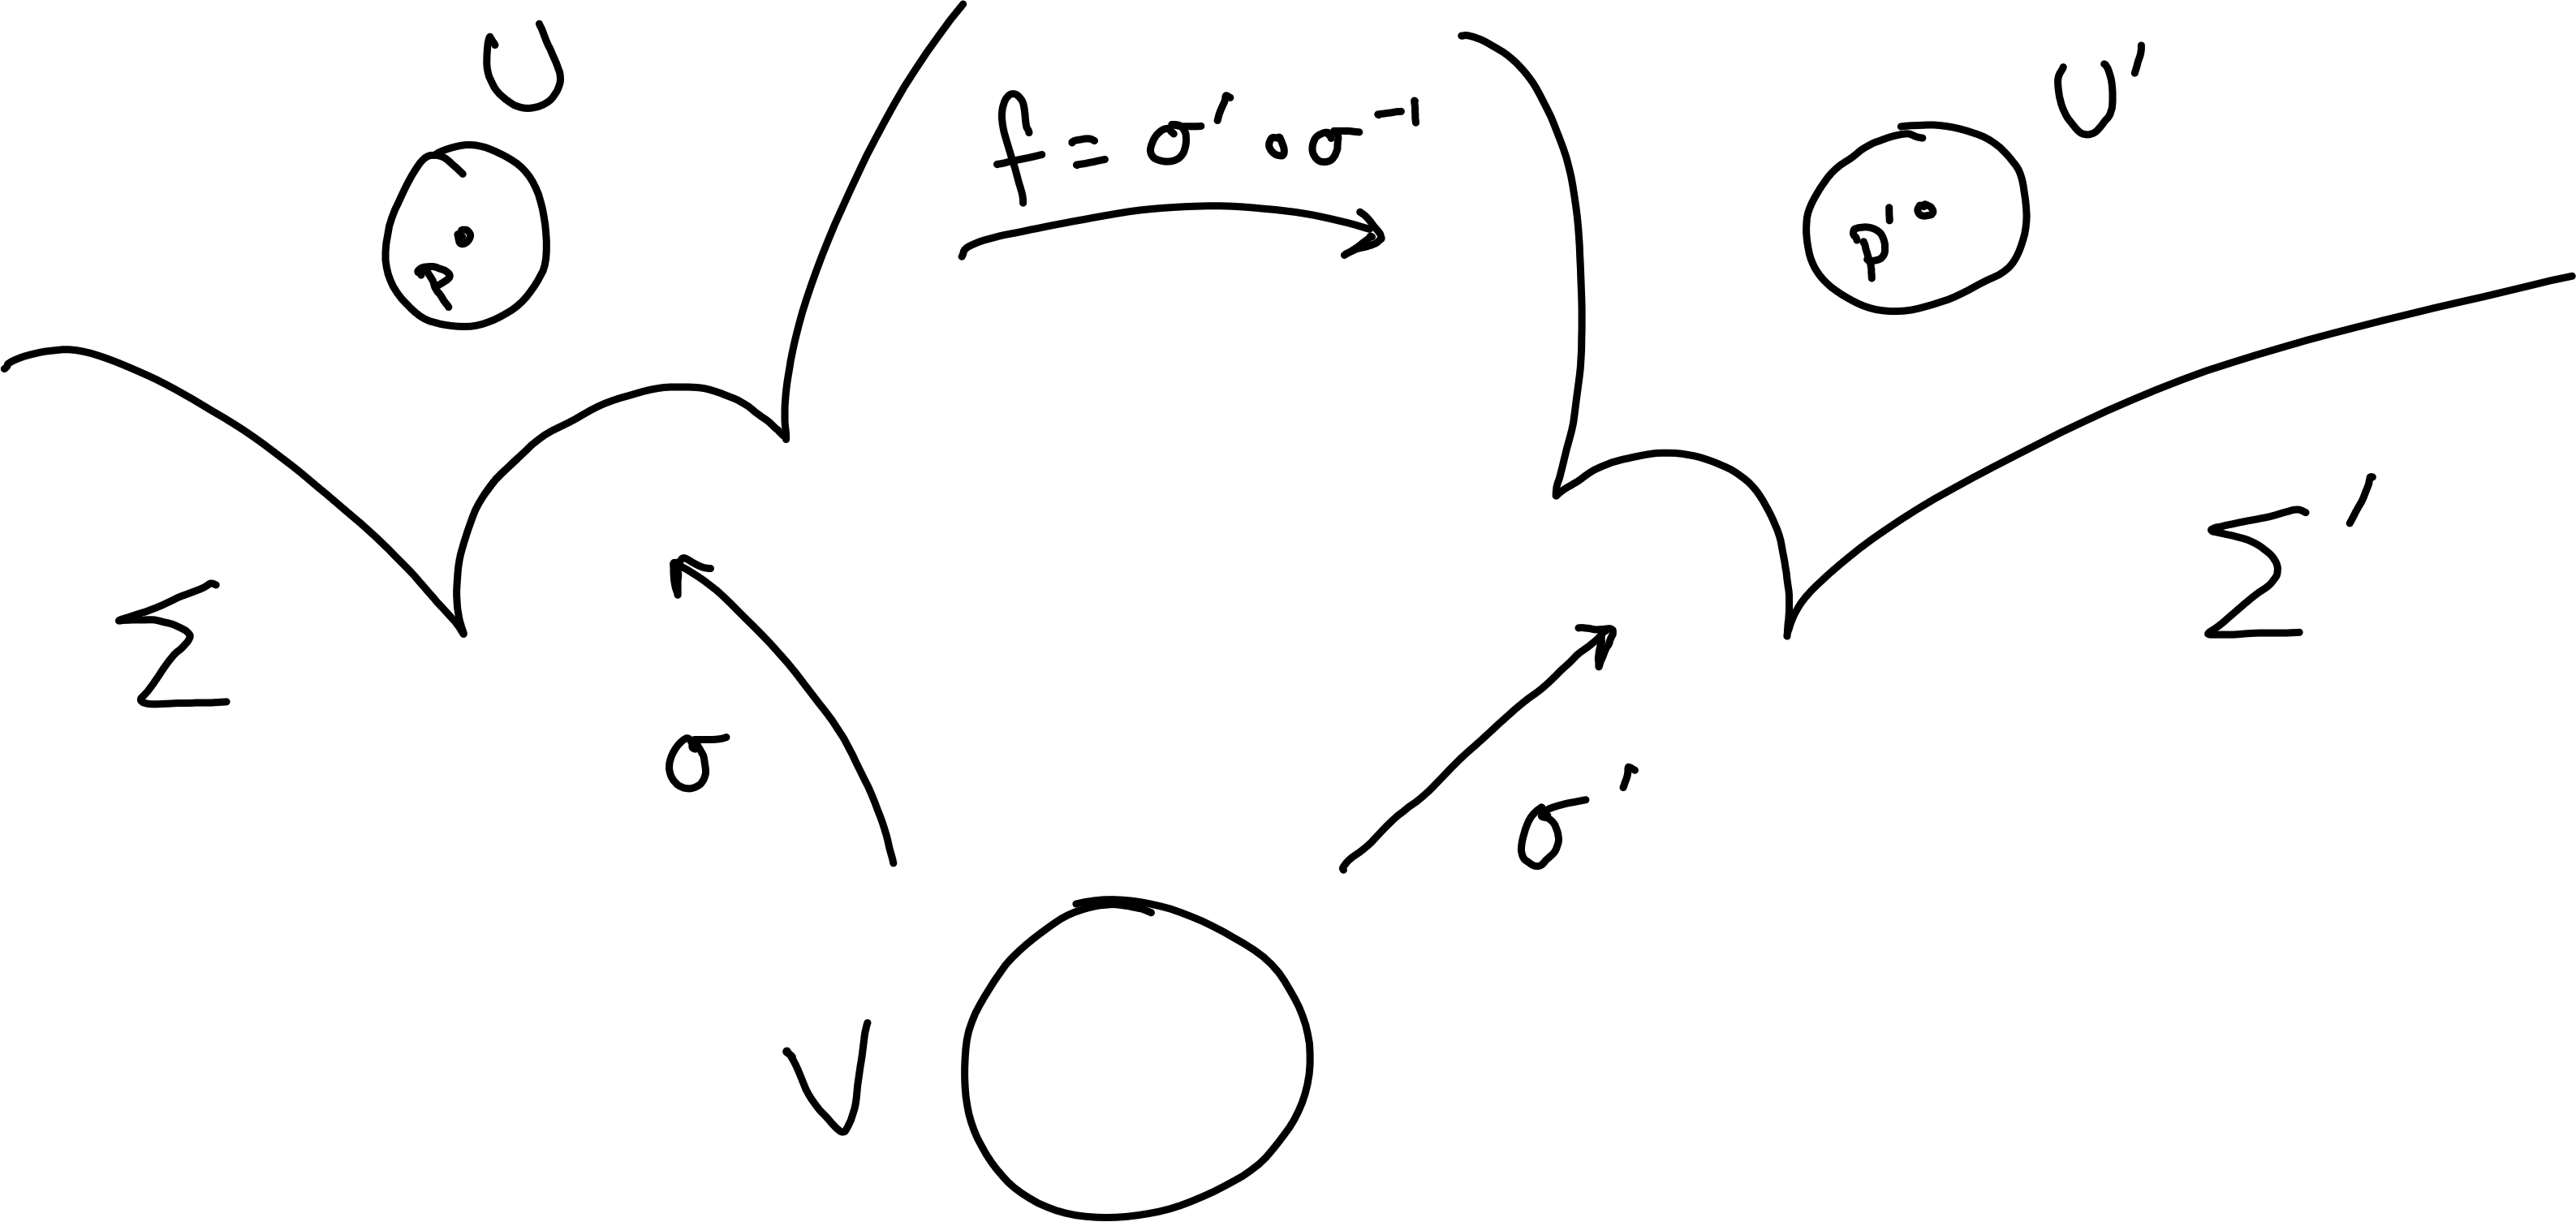
\includegraphics[height=5cm]{04-locallyIsometric} 
\end{figure}

\begin{proof}
	By definition, the first fundamental form of $\Sigma$ determines the lengths of all curves on $\Sigma$ that lie in $\sigma(V) = U$.

	$(\Longleftarrow)$: If we have $\sigma$ and $\sigma'$ with equal fundamental forms, then $\sigma' \circ \sigma\inv : U \to U'$ is an isometry since given curve $\gamma(t)$
	\begin{align*}
		\sigma\inv(\gamma(t)) &= (u(t), v(t)) \\
		\norm{\frac{d}{dt} \underbracket{\sigma' \circ \sigma\inv}_f \circ \gamma}^2 &= \norm{\frac{d}{dt} \sigma'(u(t), v(t))}^2 \\
		&= E' \dot{u}^2 + 2 F' \dot{u} \dot{v} + G' \dot{v}^2 \\
		&= E \dot{u}^2 + 2 F \dot{u} \dot{v} + G \dot{v}^2 \\
		&= \norm{\frac{d}{dt} \gamma(t)}^2 \\
		\therefore L(\sigma' \circ \sigma\inv \circ \gamma) &= L(\gamma).
	\end{align*} 

	$(\implies)$: We shall first show that the lengths of curves in $U$ determine the first fundamental form of $\sigma$.
	Given $\sigma \colon V \to U$, without loss of generality let $V = B(0,\delta)$ for some $\delta > 0$, where $\sigma(0) = p$.
	Consider, for all $\varepsilon < \delta$, the curve
	\begin{align*}
		\gamma_\varepsilon \colon [0,\varepsilon] \to U;\quad t \mapsto \sigma(t,0)
	\end{align*}
	Then,
	\begin{align*}
		\dv{\varepsilon} L(\gamma_\varepsilon) = \dv{\varepsilon} \int_0^\varepsilon \sqrt{E(t,0)} \dd{t} = \sqrt{E(\varepsilon,0)}
	\end{align*}
	Hence,
	\begin{align*}
		\eval{\dv{\varepsilon}}_{\varepsilon = 0} L(\gamma_\varepsilon) = \sqrt{E(0,0)}
	\end{align*}
	So we can determine $E$ at $p$ by looking at lengths of curves.
	We can similarly consider
	\begin{align*}
		\chi_\varepsilon \colon [0,\varepsilon] \to U;\quad t \mapsto \sigma(0,t)
	\end{align*}
	which determines $G$.
	Finally, consider
	\begin{align*}
		\lambda_\varepsilon \colon [0,\varepsilon] \to U;\quad t \mapsto \sigma(t,t)
	\end{align*}
	which determines $\sqrt{(E+2F+G)(0,0)}$ which gives $F$ implicitly.

	So if $f: U \to U'$ is a local isometry take any allowable parametrisation $\sigma' : V \to U'$ then $ = f\inv \circ \sigma'$ is s.t. the first fundamental form of $\sigma, \sigma'$ agree.
\end{proof}

\begin{example}
	Consider the cone with angle $\arctan a$ to the vertical.
	{\par
		\centering 
		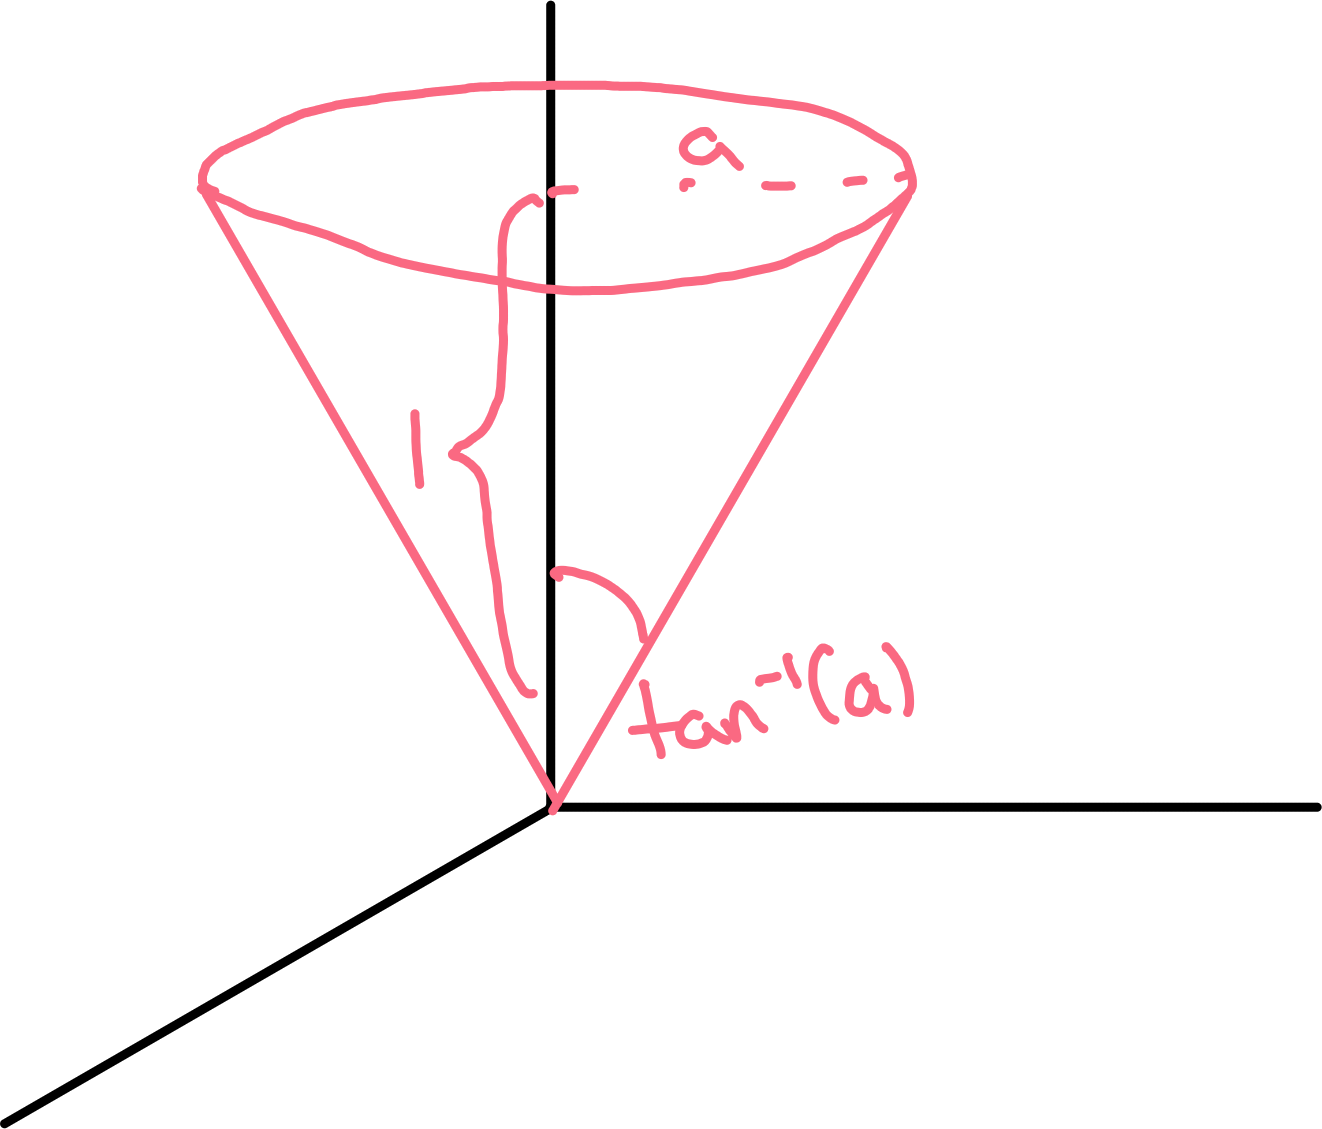
\includegraphics[height=5cm]{04-cone} 
	\par}
	For $u > 0$ and $v \in (0,2\pi)$, we define
	\begin{align*}
		\sigma(u,v) = (au\cos v, au\sin v, u).
	\end{align*}
	This parametrises the cone excluding the line at $v = 0$. \\
	The first fundamental form is
	\begin{align*}
		(1+a^2)\dd{u}^2 + a^2 u^2 \dd{v}^2
	\end{align*}
	Consider cutting the cone along the line $v = 0$ and flattening it into a plane sector.
	{\par
		\centering 
		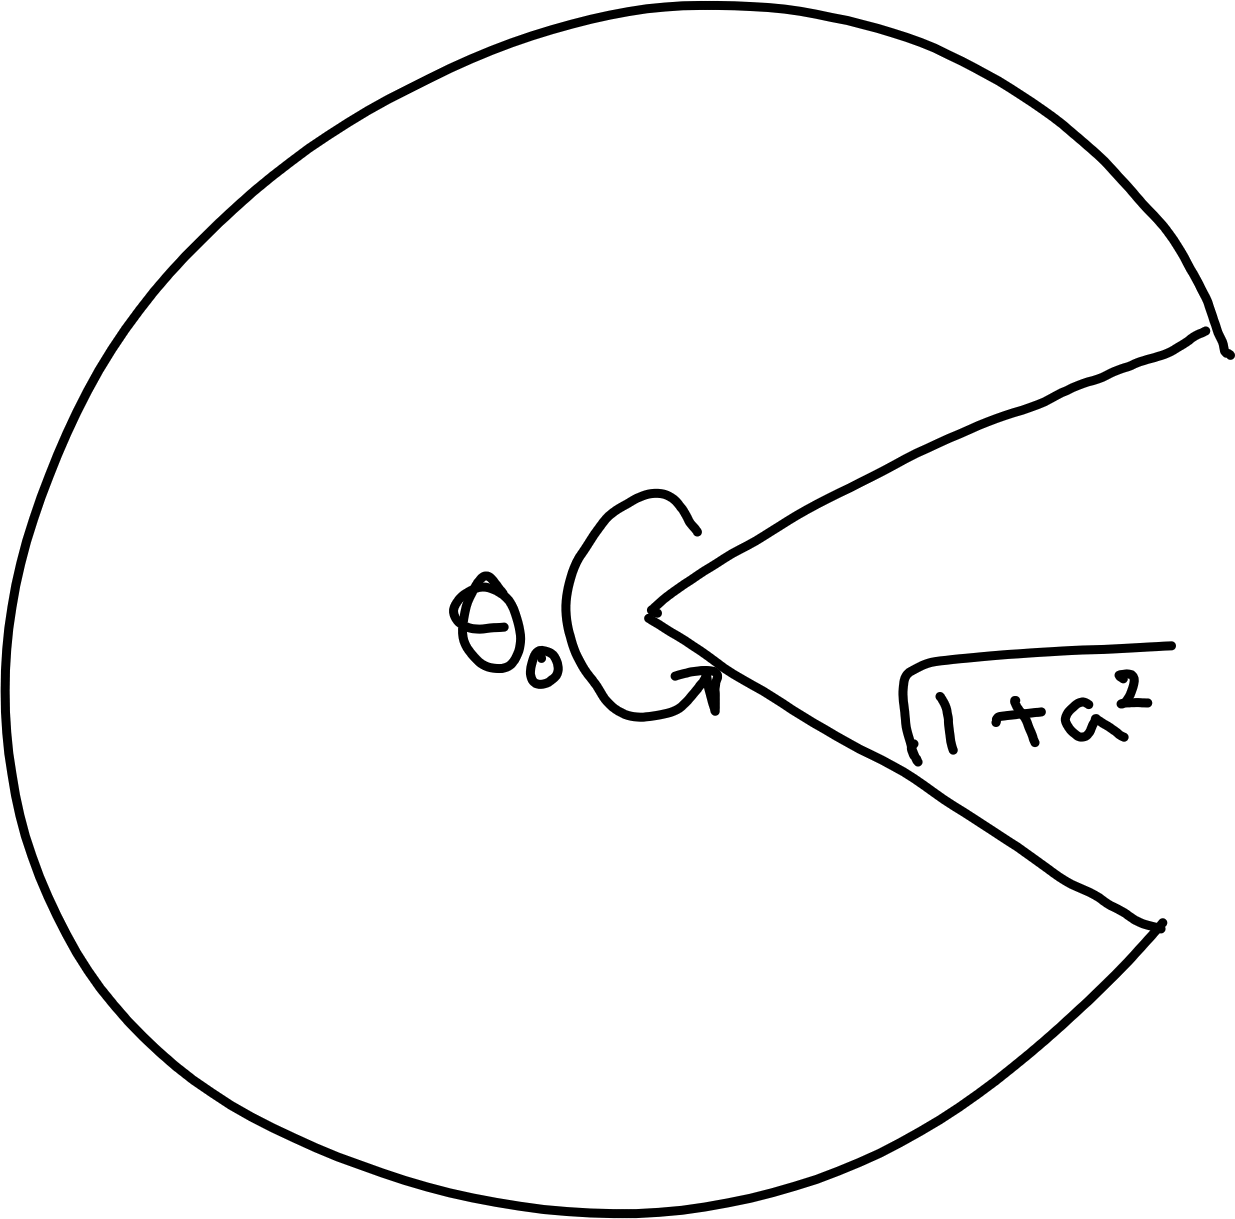
\includegraphics[height=5cm]{04-cone-unrolled} 
	\par}
	The circumference of the sector is $2 \pi a$ and the radius is $\sqrt{1+a^2}$, hence the angle traced out by the sector is $\theta_0 = \frac{2 \pi a}{\sqrt{1+a^2}}$.
	We can parametrise this subset of the plane by
	\begin{align*}
		\sigma(r,\theta) = \qty(\sqrt{1+a^2} r\cos\qty(\frac{a\theta}{\sqrt{1+a^2}}), \sqrt{1+a^2} r\sin\qty(\frac{a\theta}{\sqrt{1+a^2}}), 0)
	\end{align*}
	for $r > 0$ and $\theta \in (0,2\pi)$.
	We can then check that the first fundamental form here is
	\begin{align*}
		(1+a^2) \dd{r}^2 + r^2 a^2 \dd{\theta}^2
	\end{align*}
	which matches the first fundamental form for the cone itself.
	Hence the cone and the plane are locally isometric.

	However, the cone and plane are not globally isometric, since the two topological spaces are not homeomorphic, so no diffeomorphism that preserves lengths can be constructed.
	An intuitive way to think about this is that the cone doesn't include the origin so shrinking any curve on the cone to $0$ leaves the cone whilst the same is not true in the plane, this is the notion of simple connectedness.
\end{example}

\begin{example}
	The sphere of radius $a$, given by $\qty{x^2 + y^2 + z^2 = a^2}$, has an open set with allowable parametrisation
	\begin{align*}
		\sigma(u,v) = (a\cos u \cos v, a \cos u \sin v, a \sin u)
	\end{align*}
	where $u \in \qty(-\frac{\pi}{2}, \frac{\pi}{2})$ and $v \in (0,2\pi)$.
	This parametrises the complement of a half great circle.
	Here,
	\begin{align*}
		\sigma_u = (-a \sin u \cos v, -a \sin u \sin v, a \cos u);\quad \sigma_v = (-a \cos u \sin v, a \cos u \cos v, 0)
	\end{align*}
	Hence,
	\begin{align*}
		E = a^2; \quad F = 0;\quad G = a^2 \cos^2 u
	\end{align*}
	which gives the first fundamental form as
	\begin{align*}
		a^2 \dd{u}^2 + a^2 \cos^2 u \dd{v}^2
	\end{align*}
\end{example}

\begin{example}
	Consider the surface of revolution given by a curve
	\begin{align*}
		\eta(t) = (f(t),0,g(t))
	\end{align*}
	rotated about the $z$ axis.
	The resulting surface has parametrisation
	\begin{align*}
		\sigma(u,v) = (f(u) \cos v, f(u) \sin v, g(u))
	\end{align*}
	Hence,
	\begin{align*}
		\sigma_u = (f_u \cos v, f_u \sin v, g_u);\quad \sigma_v = (-f \sin v, f \cos v, 0)
	\end{align*}
	which gives
	\begin{align*}
		(f_u^2 + g_u^2) \dd{u}^2 + f^2 \dd{v}^2
	\end{align*}
\end{example}

\begin{lemma} \label{lem:2.3}
	Let $\Sigma$ be a smooth surface in $\mathbb R^3$, and let $p \in \Sigma$.
	Suppose we have two allowable parametrisations $\sigma \colon V \to U$ and $\sigma' \colon V' \to U$ s.t. $\sigma(0) = \sigma'(0) = p$ and U an open nbd of $p$.
	The two parametrisations differ by a transition map $f = {\sigma'}^{-1} \circ \sigma$ which is a diffeomorphism of open subsets of $\mathbb R^2$.
	There exist first fundamental forms for both parametrisations.
	Then,
	\begin{align*}
		\begin{pmatrix}
			E & F \\
			F & G
		\end{pmatrix} = (Df)^\tran \begin{pmatrix}
			E' & F' \\
			F' & G'
		\end{pmatrix} (Df)
	\end{align*}
\end{lemma}

\begin{proof}
	By definition,
	\begin{align*}
		\begin{pmatrix}
			E & F \\
			F & G
		\end{pmatrix} = \begin{pmatrix}
			\sigma_u \cdot \sigma_u & \sigma_u \cdot \sigma_v \\
			\sigma_v \cdot \sigma_u & \sigma_v \cdot \sigma_v
		\end{pmatrix} = (D\sigma)^\tran (D\sigma)
	\end{align*}
	Since, $\sigma = \sigma' \circ F \implies D \sigma = D \sigma' Df$ so $(D\sigma)^\tran (D\sigma) = (D \sigma = D \sigma' Df)^\tran (D \sigma = D \sigma' Df) = (Df)^\tran (D\sigma')^\tran (D\sigma') (Df)$.
\end{proof}

\subsection{Conformality}
If $v,w \in \mathbb R^3$, we have $v \cdot w = \norm{v} \cdot \norm{w} \cdot \cos\theta$.
This allows us to deduce the angle $\theta$ between two vectors given their dot product and lengths.
This can also be done when $v,w$ are in the tangent plane $T_p \Sigma$, and then we can express the angle in terms of the first fundamental form.
Let $\sigma$ be an allowable parametrisation for $\Sigma$ near $p$, such that $D\eval{\sigma}_0$ evaluates to $v$ at $v_0$ and $w$ at $w_0$.
\begin{align*}
	\cos \theta &= \frac{v \cdot w}{\norm{v} \cdot \norm{w}} = \frac{I(v_0, w_0)}{\sqrt{I(v_0,v_0)} \sqrt{I(w_0,w_0)}} \\
	I(v_0, w_0) &= v_0^\tran \begin{pmatrix}
		E & F \\
		F & G
	\end{pmatrix} w_0.
\end{align*}
where $I$ denotes the first fundamental form of $\sigma$ at zero.

\begin{lemma}
	Let $\Sigma$ be a smooth surface in $\mathbb R^3$, and let $\sigma \colon V \to U$ be an allowable parametrisation of $\Sigma$ near $p$. \\
	Then $\sigma$ is \textit{conformal} (preserves angles) iff $E = G$ and $F = 0$ in the first fundamental form.
\end{lemma}

\begin{proof}
	$(\implies)$: Consider curves $\gamma \colon t \mapsto (u(t), v(t))$ and $\widetilde \gamma \colon t \mapsto (\widetilde u(t), \widetilde v(t))$ in $V$, where $\gamma(0) = \widetilde \gamma(0) = 0 \in V$.
	Let $\sigma$ be a parametrisation $V \to U \subset \Sigma$ such that $\sigma(0) = p \in \Sigma$.
	Then the curves $\sigma \circ \gamma$ and $\sigma \circ \widetilde \gamma$ meet at angle $\theta$ on $\Sigma$, where
	\begin{align*}
		\cos \theta = \frac{E \dot u \dot {\widetilde u} + F \qty(\dot u \dot{\widetilde v} + \dot v \dot{\widetilde u}) + G \dot v \dot{\widetilde v}}{\sqrt{E \dot u^2 + 2F \dot u \dot v + G \dot v^2} \sqrt{E \dot{\widetilde u}^2 + 2F \dot{\widetilde u} \dot {\widetilde v} + G \dot{\widetilde v}^2}}
	\end{align*}
	In particular, if $\sigma$ is conformal, suppose $\gamma(t) = (t,0)$ and $\widetilde \gamma(t) = (0,t)$.
	Then, we have that the curves meet at $\frac{\pi}{2}$ in $V$, so they meet at $\frac{\pi}{2}$ in $\Sigma$, so we find that $\cos \theta = 0 \implies F = 0$ as $\dot{u} = \dot{\widetilde v} = 1$ and $\dot{\widetilde u} = \dot{v} = 0$. \\
	Similarly, if $\gamma(t) = (t,t)$ and $\widetilde \gamma(t) = (t,-t)$, we find $\cos \theta = 0 \implies E = G$.

	$(\Longleftarrow)$: Conversely, suppose there exists a parametrisation $\sigma$ such that $E = G$ and $F = 0$.
	Then, in this parametrisation, the first fundamental form is of the form $\rho \qty(\dd{u}^2 + \dd{v}^2)$ for $\rho = E \colon V \to \mathbb R$.
	So \begin{align*}
		\cos \theta = \frac{\dot u \dot {\widetilde u} + \dot v \dot{\widetilde v}}{\sqrt{\dot u^2 + \dot v^2} \sqrt{\dot{\widetilde u}^2 + \dot{\widetilde v}^2}},
	\end{align*} i.e. angles don't change.

	Alternatively, the first fundamental form is a pointwise rescaling of the Euclidean fundamental form $\dd{u}^2 + \dd{v}^2$.
	Rescaling the plane does not change angles, so $\sigma$ is conformal as required.
\end{proof}

\begin{remark}
	Conformality in charts is historically important for cartography.
	The existence of conformal charts is closely connected to Riemann surfaces, which are topological surfaces locally modelled on $\mathbb C$ instead of $\mathbb R^2$.
\end{remark}

\subsection{Area}
Recall that a parallelogram spanned by vectors $v, w$ has area \\$\norm{v \times w} = \sqrt{\inner{v,v}\inner{w,w} - \inner{v,w}^2}$, where $\times$ denotes the cross product.
Let $\sigma \colon V \to U \subset \Sigma$ be an allowable parametrisation with $\sigma(0) = p$, and consider $\sigma_u, \sigma_v \in T_p \Sigma$.
The square of the area of the infinitesimal parallelogram spanned by $\sigma_u, \sigma_v$ is given by
\begin{align*}
	\qty(\inner{\sigma_u, \sigma_u}\inner{\sigma_v, \sigma_v} - \inner{\sigma_u, \sigma_v}^2)^{1 / 2} = \sqrt{EG - F^2}.
\end{align*}

\begin{definition}[Area]
	Let $\Sigma$ be a smooth surface in $\mathbb R^3$, and $\sigma \colon V \to U \subset \Sigma$ an allowable parametrisation.
	Then,
	\begin{align*}
		\mathrm{area}(U) = \int_V \sqrt{EG - F^2} \dd{u}\dd{v}
	\end{align*}
\end{definition}

\begin{remark}
	This is independent of parametrisation.
	Indeed, suppose $\sigma \colon V \to U$ and $\widetilde \sigma \colon \widetilde V \to U$ are allowable.
	Then $\widetilde \sigma = \sigma \circ \varphi$ for some transition map $\varphi = \sigma\inv \circ \widetilde \sigma \colon \widetilde V \to V$.
	We know then that by \Cref{lem:2.3}
	\begin{align*}
		\begin{pmatrix}
			\widetilde E & \widetilde F \\
			\widetilde F & \widetilde G
		\end{pmatrix} = (D\widetilde \sigma)^\tran (D\widetilde \sigma) = (D\varphi)^\tran \begin{pmatrix}
			E & F \\
			F & G
		\end{pmatrix} (D\varphi)
	\end{align*}
	Hence by taking determinants,
	\begin{align*}
		\sqrt{\widetilde E \widetilde G - \widetilde F^2} = \abs{\det(D\varphi)} \sqrt{EG - F^2}
	\end{align*}
	The usual change of variables formula for integration, combined with the fact that $\varphi$ is a diffeomorphism, gives
	\begin{align*}
		\int_V \sqrt{EG - F^2} \dd{u}\dd{v} = \int_{\widetilde V} \sqrt{\widetilde E \widetilde G - \widetilde F^2} \dd{\widetilde u}\dd{\widetilde v}.
	\end{align*}
	So $\operatorname{area}(U)$ is intrinsic and well-defined.

	Note, we can compute the area of an open set $U \subset \Sigma$, not necessarily lying in a single parametrisation, by covering the set by a finite amount of open subsets which lie in single charts.
	For instance, if $\Sigma$ is compact, we can compute the area of $\Sigma$ itself.
\end{remark}

\begin{example}
	Consider the graph $\Sigma = \qty{(u,v,f(u,v)) \colon (u,v) \in \mathbb R^2}$, where $f \colon \mathbb R^2 \to \mathbb R$ is a smooth function.
	This has a global parametrisation $\sigma(u,v) = (u,v,f(u,v))$.
	Here, $\sigma_u = (1,0,f_u)$ and $\sigma_v = (0,1,f_v)$, hence
	\begin{align*}
		\sqrt{EG - F^2} = \sqrt{1+f_u^2+f_v^2}
	\end{align*}
	Let $U_R \subset \Sigma$ be the part of the graph lying inside the disc $B(0,R) \subset \mathbb R^2$.
	Then
	\begin{align*}
		\mathrm{area}(U_R) = \int_{B(0,R)} \sqrt{1+f_u^2+f_v^2} \dd{u}\dd{v} \geq \pi R^2
	\end{align*}
	with equality exactly when $f_u = f_v = 0$, which is when $f$ is constant and $U_R$ is contained inside a plane perpendicular to the $z$ axis.
	Hence, the projection from $\Sigma$ to $\mathbb R^2_{xy}$ is not area-preserving, unless $\Sigma$ is a plane perpendicular to the $z$ axis.
\end{example}

\begin{example}
	Consider the sphere enclosed exactly by a cylinder.
	The cylindrically radial projection from the sphere to the cylinder is area-preserving.
	You will prove this in Sheet 2.
\end{example}

\subsection{Second fundamental form}
Let $\sigma \colon V \to U \subset \Sigma$ be allowable.
By using Taylor's theorem, we can write
\begin{align*}
	\sigma(u+h,v+\ell) = \sigma(u,v) + h \sigma_u(u,v) + \ell \sigma_v(u,v) + \frac{1}{2} \qty(h^2 \sigma_{uu}(u,v) + 2h\ell \sigma_{uv}(u,v) + \ell^2 \sigma_{vv}(u,v)) + O(h^3,\ell^3)
\end{align*}
where $h,\ell$ are small, and $(u+h,v+\ell) \in V$.
Recall that if $p = \sigma(u,v)$, we have $T_p \Sigma = \genset{\qty{\sigma_u,\sigma_v}}$.
Hence, the orthogonal distance from $\sigma(u+h,v+\ell)$ to the affine tangent plane $T_p \Sigma + p$ is given by projection to the normal direction.
\begin{align*}
	\inner{n,\sigma(u+h,v+\ell) - \sigma(u,v)} = \frac{1}{2} \qty(\inner{n,\sigma_{uu}} h^2 + 2\inner{n,\sigma_{uv}} h\ell + \inner{n,\sigma_{vv}}\ell^2) + O(h^3,\ell^3)
\end{align*}
\begin{definition}
	The \textit{second fundamental form} of $\Sigma$ in the allowable parametrisation $\sigma$ is the quadratic form
	\begin{align*}
		L \dd{u}^2 + 2 M \dd{u} \dd{v} + N \dd{v}^2
	\end{align*}
	where
	\begin{align*}
		L = \inner{n,\sigma_{uu}};\quad M = \inner{n,\sigma_{uv}};\quad N = \inner{n,\sigma_{vv}}
	\end{align*}
	and
	\begin{align*}
		n = \frac{\sigma_u \times \sigma_v}{\norm{\sigma_u \times \sigma_v}}
	\end{align*}
	We can write this as the matrix
	\begin{align*}
		\begin{pmatrix}
			L & M \\
			M & N
		\end{pmatrix}
	\end{align*}
	which defined a quadratic form on $T_p \Sigma$ which varies smoothly in $p$.
\end{definition}
\begin{lemma}
	Let $V$ be connected and $\sigma \colon V \to U \subset \Sigma$ be an allowable parametrisation such that the second fundamental form vanishes identically with respect to $\sigma$.
	Then $U$ lies in an affine plane.
\end{lemma}
\begin{remark}
	The first fundamental form is a non-degenerate symmetric bilinear form on $T_p \Sigma$, whereas the second fundamental form may be degenerate.
\end{remark}
\begin{proof}
	By definition,
	\begin{align*}
		\inner{n,\sigma_u} = 0 = \inner{n,\sigma_v}
	\end{align*}
	Hence, by differentiating, we find
	\begin{align*}
		0 = \inner{n_u, \sigma_u} + \inner{n, \sigma_{uu}} = \inner{n_v, \sigma_v} + \inner{n, \sigma_{vv}} = \inner{n_v, \sigma_u} + \inner{n,\sigma_{uv}}
	\end{align*}
	Some of these terms appear in the definition of the second fundamental form:
	\begin{align*}
		L = \inner{n,\sigma_{uu}} = -\inner{n_u, \sigma_u};\quad M = \inner{n,\sigma_{uv}} = -\inner{n_v, \sigma_u} = -\inner{n_u, \sigma_v};\quad N = \inner{n,\sigma_{vv}} = -\inner{n_v, \sigma_v}
	\end{align*}
	If the second fundamental form vanishes, then $n_u$ is orthogonal to $\sigma_u$, $\sigma_v$, and $n$ itself.
	Since $\sigma_u, \sigma_v, n$ form a basis for $\mathbb R^3$, we have $n_u = 0$.
	Similarly, $n_v = 0$, hence $n$ is constant by the mean value theorem.
\end{proof}
\begin{remark}
	The first fundamental form in parametrisation $\sigma$ can be written $(D \sigma)^\tran (D \sigma)$.
	We can similarly write the second fundamental form as
	\begin{align*}
		-(Dn)^\tran (D\sigma) = \begin{pmatrix}
			L & M \\
			M & N
		\end{pmatrix} = -\begin{pmatrix}
			n_u \cdot \sigma_u & n_u \cdot \sigma_v \\
			n_v \cdot \sigma_u & n_v \cdot \sigma_v
		\end{pmatrix}
	\end{align*}
	Hence, if $\sigma \colon V \to \Sigma$ and $\widetilde \sigma \colon \widetilde V \to \Sigma$ are allowable parametrisations for an open set $U \subset \Sigma$ with transition map $\varphi \colon \widetilde V \to V$ given by $\varphi = \sigma^{-1} \circ \widetilde \sigma$, we can use the above expression to find
	\begin{align*}
		\begin{pmatrix}
			\widetilde L & \widetilde M \\
			\widetilde M & \widetilde N
		\end{pmatrix} = \pm (D\varphi)^\tran \begin{pmatrix}
			L & M \\
			M & N
		\end{pmatrix} (D\varphi)
	\end{align*}
	The change in sign depends on whether the transition map preserves or reverses orientation.
	If the normal vectors agree, there is no negative sign.
	\begin{align*}
		\eval{n_{\sigma \circ \varphi}}_{(\widetilde u, \widetilde v)} = \pm \eval{n_\sigma}_{\varphi(\widetilde u, \widetilde v)}
	\end{align*}
	for $(\widetilde u, \widetilde v) \in \widetilde V$.
	In particular, if $\det (D \varphi) < 0$, we arrive at a negative sign.
	If we assume that $V, \widetilde V$ are connected, the determinant $\det (D \varphi)$ does not change sign.
\end{remark}
\begin{example}
	Consider the cylinder with allowable parametrisation
	\begin{align*}
		\sigma(u,v) = (a \cos u, a \sin u, v)
	\end{align*}
	where $u \in (0,2\pi), v \in \mathbb R$.
	Note that $\sigma_{uv} = \sigma_{vv} = 0$, hence $M = N = 0$.
	We can show that the second fundamental form is given by
	\begin{align*}
		\begin{pmatrix}
			-a & 0 \\
			0  & 0
		\end{pmatrix};\quad -a \dd{u}^2
	\end{align*}
\end{example}

\subsection{Gauss maps}
\begin{definition}
	Let $\Sigma$ be a smooth oriented surface in $\mathbb R^3$.
	The \textit{Gauss map} $n \colon \Sigma \to \mathbb S^2$ is the map $p \mapsto n(p)$, where the normal vector is normalised and hence lies in the unit sphere.
\end{definition}
\begin{lemma}
	The Gauss map is smooth.
\end{lemma}
\begin{proof}
	Since smoothness is a local property, it suffices to check the smoothness of the map on an arbitrary parametrised part of $\Sigma$.
	Let $\sigma \colon V \to U \subset \Sigma$ be allowable and compatible with a chosen orientation.
	Then
	\begin{align*}
		n(p) = \frac{\sigma_u \times \sigma_v}{\norm{\sigma_u \times \sigma_v}}
	\end{align*}
	Since $\sigma$ is allowable, the denominator is non-vanishing.
	Hence, $n(p)$ is smooth as required.
\end{proof}
\begin{remark}
	If $\Sigma = F^{-1}(0)$ for some function $F \colon \mathbb R^3 \to \mathbb R$ with nonzero derivative $DF$ at all points $x \in \Sigma$ (which was required for $\Sigma$ to be a smooth surface in $\mathbb R^3$), then we can explicitly calculate the Gauss map to be
	\begin{align*}
		n(p) = \frac{\grad F}{\norm{\grad F}}
	\end{align*}
	Note that,
	\begin{align*}
		T_p \Sigma = T_{n(p)} S^2 = (n(p))^\perp
	\end{align*}
	since the two planes are orthogonal to the same vector.
	More concretely, if $v \in T_p \Sigma$ is $\gamma'(0)$ where $\gamma \colon (-\varepsilon, \varepsilon) \to \Sigma$, $\gamma(0) = p$ for a smooth curve $\gamma$, we can apply the Gauss map to $\gamma$ and find
	\begin{align*}
		n \circ \gamma \colon (-\varepsilon, \varepsilon) \to S^2;\quad (n \circ \gamma)(0) = n(p)
	\end{align*}
	Then, by the chain rule,
	\begin{align*}
		D\eval{n}_p(v) = (n \circ \gamma)'(0) \in T_{n(p)} S^2 = T_p \Sigma
	\end{align*}
	Thus, the derivative of the Gauss map is $D\eval{n}_p \colon T_p \Sigma \to T_p \Sigma$.
	This can be viewed as an endomorphism of a fixed (with respect to parametrisation choice) two-dimensional subspace of $\mathbb R^3$.

	To summarise, let $\Sigma$ be an oriented smooth surface in $\mathbb R^3$.
	Then,
	\begin{enumerate}
		\item The first fundamental form is a symmetric bilinear form $\inner{\wildcard,\wildcard} = \Iff_p \colon T_p \Sigma \times T_p \Sigma \to \mathbb R$, which is the restriction of the Euclidean inner product to this space $T_p \Sigma$.
		      We can write $\Iff_p(v,w)$, where $v, w \in T_p \Sigma$.
		\item The second fundamental form is also a symmetric bilinear form $\IIff_p \colon T_p \Sigma \times T_p \Sigma \to \mathbb R$, given by
		      \begin{align*}
			      \IIff_p(v,w) = \Iff_p\qty(-D\eval{n}_p(v), w)
		      \end{align*}
		      where $n$ is the Gauss map.
	\end{enumerate}
	If we choose an allowable parametrisation (which for the second fundamental form must be correctly oriented) $\sigma \colon V \to U \subset \Sigma$ near $p \in \Sigma$, and if
	\begin{align*}
		D \eval{\sigma}_0(\hat v) = v;\quad D \eval{\sigma}_0(\hat w) = w;\quad \sigma(0) = p
	\end{align*}
	Then,
	\begin{align*}
		\Iff_p(v,w) = {\hat v}^\tran \begin{pmatrix}
			E & F \\
			F & G
		\end{pmatrix} \hat w;\quad \IIff_p(v,w) = {\hat v}^\tran \begin{pmatrix}
			L & M \\
			M & N
		\end{pmatrix} \hat w
	\end{align*}
	where $E, F, G, L, M, N$ depend on the choice of $\sigma$.
	Note that the functions $\Iff_p$ and $\IIff_p$ are independent of $\sigma$.
\end{remark}
\begin{lemma}
	The derivative of the Gauss map is self-adjoint.
	More precisely, viewing $D \eval{n}_p \colon T_p \Sigma \to T_p \Sigma$ as an endomorphism over the inner product space with the first fundamental form, this linear map satisfies
	\begin{align*}
		\Iff_p\qty(D \eval{n}_p(v), w) = \Iff_p\qty(v, D \eval{n}_p(w))
	\end{align*}
	for all $v, w \in T_p \Sigma$.
\end{lemma}
\begin{proof}
	From expressions for local parametrisations, we can show that $\Iff_p$ and $\IIff_p$ are symmetric.
	Hence,
	\begin{align*}
		\Iff_p(D\eval{n}_p(v),w) = -\IIff_p(v,w) = -\IIff_p(w,v) = \Iff_p(D \eval{n}_p(w),v) = \Iff_p(v,D\eval{n}_p(w))
	\end{align*}
\end{proof}
\begin{remark}
	The \textit{fundamental theorem of surfaces in $\mathbb R^3$} states that a smooth oriented connected surface in $\mathbb R^3$ is determined completely, up to rigid motion, by the two fundamental forms.
\end{remark}

\subsection{Gauss curvature}
\begin{definition}
	Let $\Sigma$ be a smooth surface in $\mathbb R^3$.
	The \textit{Gauss curvature} $\kappa \colon \Sigma \to \mathbb R$ of $\Sigma$ is the function defined by
	\begin{align*}
		\kappa(p) = \det(D \eval{n}_p)
	\end{align*}
\end{definition}
\begin{remark}
	This is always well-defined, even if $\Sigma$ is not oriented.
	This is because $\Sigma$ is always locally orientable, and the two normals differ by sign.
	In two dimensions, $\det(-A) = \det(A)$, so the determinant is invariant.
\end{remark}
We can compute $\kappa$ directly.
Let $\Sigma$ be a smooth surface in $\mathbb R^3$, and $\sigma$ an allowable parametrisation for an open neighbourhood of a point $p$.
Recall that
\begin{align*}
	\Iff_p \colon T_p \Sigma \to T_p \Sigma;\quad (v,w) \mapsto \inner{v,w};\quad \IIff_p \colon T_p \Sigma \to T_p \Sigma;\quad (v,w) \mapsto \Iff_p(-\eval{Dn}_p(v), w)
\end{align*}
and $\eval{Dn}_p \colon T_p \Sigma \to T_p \Sigma$.
The choice of parametrisation $\sigma$ for an open neighbourhood $U$ of $p$ provides a preferred basis $\qty{\sigma_u, \sigma_v}$ for $T_p \Sigma$.
We can therefore write the fundamental forms as matrices with respect to this basis.
Let $A = \Iff_p, B = \IIff_p, \mathbb S = \eval{Dn}_p$ in this basis.
In matrix form, we can write $\IIff_p = \Iff_p(-\eval{Dn}_p(v),w)$ as
\begin{align*}
	B = -\mathbb S^\tran A \implies \kappa(p) = \det(\mathbb S) = \det(-A^{-1}B) = \frac{LN-M^2}{EG-F^2}
\end{align*}
If $\sigma, \widetilde \sigma$ are allowable and $\varphi = \sigma^{-1} \circ \sigma$ is a transition map, then
\begin{align*}
	\widetilde A = (D\varphi)^\tran A (D \varphi);\quad \widetilde B = \pm (D\varphi)^\tran B (D \varphi)
\end{align*}
Since the sign vanishes under taking determinants, $\kappa$ is intrinsic and does not depend on the choice of parametrisation.
\begin{example}
	For a cylinder $\qty{x^2 + y^2 = 1}$ the Gauss map $n \colon \Sigma \to S^2$ has image which lies in the equator.
	Its derivative $\eval{Dn}_p \colon T_p \Sigma \to T_p \Sigma$ has one-dimensional image, since any $\gamma \colon (-\varepsilon, \varepsilon) \to \Sigma$ has $n \circ \gamma \subset S^1$.
	Hence its Gauss curvature is zero.
\end{example}
\begin{definition}
	A smooth surface in $\mathbb R^3$ with vanishing Gauss curvature everywhere is \textit{flat}.
\end{definition}
\begin{remark}
	If $\sigma\colon V \to U$ is allowable, and $n_\sigma$ is defined to be $n \circ \sigma \colon V \to S^2$, then
	\begin{align*}
		\eval{Dn_\sigma}_0 \colon \sigma_u \mapsto (n_\sigma)_u;\quad \sigma_v \mapsto (n_\sigma)_v
	\end{align*}
	In particular, $\kappa(p) = \kappa(\sigma(0))$ vanishes if and only if $(n_\sigma)_u \times (n_\sigma)_v = 0$.
	Usually, we will write $n$ to denote $n_\sigma$.
	In this case, the condition for flatness is that $n_u \times n_v = 0$.
\end{remark}
\begin{example}
	If $\Sigma$ is the graph of a smooth function $f$, then on the example sheets we show that
	\begin{align*}
		\kappa = \frac{f_{uu} f_{vv} - f_{uv}^2}{(1+f_u^2 + f_v^2)^2}
	\end{align*}
	Hence, the curvature depends on the derivative and the Hessian of $f$.
	For instance, let $f(u,v) = \sqrt{r^2 - u^2 - v^2}$.
	Here, the graph is a piece of a sphere of radius $r$.
	We can find
	\begin{align*}
		\eval{f_{uu}}_0 = \eval{f_{vv}}_0 = \frac{-1}{r};\quad \eval{f_{uv}}_0 = 0 \implies \kappa(0,0,r) = \frac{1}{r^2}
	\end{align*}
	Since $O(3)$ acts transitively on $S^2$, and the fundamental forms are preserved by such global isometries, $\kappa = \frac{1}{r^2}$ everywhere on the sphere of radius $r$.
\end{example}
\begin{example}
	Let $\Sigma$ be the smooth surface given by $\qty{z = x^2 + y^2}$.
	We claim that, for the inward facing choice of orientation, the image of the Gauss map is the open northern hemisphere.
	Note that $\Sigma$ is invariant under rotations about the $z$ axis.
	Also, we can show that if $R$ is a rotation, $n \circ R = R \circ n$.
	Therefore, it suffices to consider an arbitrary point with $y = 0$.

	Here, $\Sigma = F^{-1}(0)$ for the function $F(x,y,z) = z - x^2 - y^2$, which has nonvanishing derivative at the points $p \in \Sigma$.
	Hence, at $p = (x,0,x^2)$, we have
	\begin{align*}
		n(p) = \frac{\grad{F}}{\norm{\grad{F}}} = \frac{(-2x,0,1)}{\sqrt{1+4x^2}}
	\end{align*}
	We can check explicitly that this map has image which an arc lying in the open northern hemisphere.
\end{example}

\subsection{Elliptic, hyperbolic, and parabolic points}
\begin{definition}
	Let $\Sigma$ be a smooth surface in $\mathbb R^3$ and $p \in \Sigma$.
	We say that $p$ is
	\begin{enumerate}
		\item \textit{elliptic} if $\kappa(p) > 0$;
		\item \textit{hyperbolic} if $\kappa(p) < 0$;
		\item \textit{parabolic} if $\kappa(p) = 0$.
	\end{enumerate}
\end{definition}
\begin{lemma}
	In a sufficiently small neighbourhood of an elliptic point $p$, $\Sigma$ lies entirely on one side of $p + T_p \Sigma$.
	If $p$ is hyperbolic, $\Sigma$ lies on both sides of $p + T_p \Sigma$.
\end{lemma}
\begin{proof}
	Let $\sigma$ be a local parametrisation near $p$.
	Here,
	\begin{align*}
		\kappa = \frac{LN-M^2}{EG-F^2}
	\end{align*}
	The denominator is always positive, since it is the determinant of a positive definite symmetric bilinear form $\Iff_p$.
	Hence, the sign of $\kappa$ depends on the sign of $LN-M^2$.
	If $w = h \sigma_u + \ell \sigma_v \in T_p \Sigma$, then $\frac{1}{2} \IIff_p(w,w)$ measures the signed distance from $\sigma(h,l)$ to $p + T_p \Sigma$.
	If $p$ is elliptic, then $\IIff_p$ has eigenvalues of the same sign, so it is either positive or negative definite at $p$.
	Since $\IIff_p$ varies smoothly in $p$, it remains positive or negative definite in a small neighbourhood of $p$.
	Hence, in such a neighbourhood, the signed distance has the same sign as required.
	Conversely, if $p$ is hyperbolic, $\IIff_p(w,w)$ takes both signs in a neighbourhood of $p$.
\end{proof}
\begin{remark}
	We cannot conclude anything about parabolic points \textit{a priori}.
	For instance, the cylinder is flat (all points are parabolic), and the surface lies on one side of the tangent plane at every point.
	Consider also the \textit{monkey saddle} defined by
	\begin{align*}
		\sigma(u,v) = (u,v,u^3 - 3v^2 u)
	\end{align*}
	which has a parabolic point at the origin, but $\Sigma$ lies on both sides of the tangent plane in every open neighbourhood of the origin.
	At $p = \sigma(0,0)$, the Gauss curvature vanishes, but the surface lies locally on both sies of the tangent plane.
\end{remark}
\begin{proposition}
	Let $\Sigma$ be a compact smooth surface in $\mathbb R^3$.
	Then $\Sigma$ has an elliptic point.
\end{proposition}
\begin{proof}
	Since $\Sigma$ is compact, it is closed and bounded as a subset of $\mathbb R^3$.
	Hence, for $R'$ sufficiently large, $\Sigma$ lies entirely within $\overline{B(0,R')}$.
	Let $R$ be the minimal such $R'$.
	Up to a global isometry of $\mathbb R^3$, there exists a point $p = (0,0,R) \in \Sigma$ on the sphere $S^2(R)$ of radius $R$.
	Here, $T_p \Sigma = T_p S^2$.
	Hence, locally near $p$, we can view $\Sigma$ as the graph of a smooth function $f \colon V \to \mathbb R^3$ on the $x, y$ coordinates with the property that $f - \sqrt{R^2 - u^2 - v^2} \leq 0$.
	This expresses the fact that $\Sigma$ lies underneath the sphere of radius $R$.

	We can now consider the Taylor series of $f$.
	Note that $(0,0)$ is a maximum point of $f$, hence $f_u = f_v = 0$ at $0$.
	Thus, for sufficiently small $u,v$,
	\begin{align*}
		\frac{1}{2} \qty(f_{uu} u^2 + 2f_{uv} uv + f_{vv} v^2) + \frac{1}{2R} (u^2 + v^2) \leq 0
	\end{align*}
	Hence, the second fundamental form is locally negative definite near $(0,0)$.
	Hence, $\kappa(p) > 0$, so $p$ is elliptic as required.
	In particular, the curvature at this point is greater than that of the sphere.
\end{proof}
\begin{theorem}
	Let $\Sigma$ be a smooth surface in $\mathbb R^3$, and let $p \in \Sigma$ such that $\kappa(p) \neq 0$.
	Let $U$ be an open neighbourhood of $p$, and a decreasing sequence $A_i \subset U$ of neighbourhoods that `shrink to $p$', in the sense that for all $\varepsilon > 0$, $A_i \subset B(p,\varepsilon)$ for sufficiently large $i$.
	Then,
	\begin{align*}
		\abs{\kappa(p)} = \lim_{i \to \infty} \frac{\mathrm{area}_{S^2} (n(A_i))}{\mathrm{area}_{\Sigma} (A_i)}
	\end{align*}
	In other words, the Gauss curvature is an infinitesimal measure of how much the Gauss map $n$ distorts area.
\end{theorem}
\begin{remark}
	Around hyperbolic points, the signed area of $n(A_i)$ is reversed, since curves $\gamma$ reverse direction under $n$.
	We can alternatively define the \textit{signed area} of $n(A_i)$ to be the area of $n(A_i)$ if $\kappa > 0$ and the negation of this area if $\kappa < 0$.
	The above theorem holds when $\kappa = 0$, but this will not be proven.
\end{remark}
\begin{proof}
	Let $\sigma$ be an allowable parametrisation near $p \in \Sigma$.
	Using $\sigma$, we can define the open sets $\sigma^{-1}(A_i) = V_i \subset V$.
	Since the $A_i$ shrink to $p$, we have that $\bigcap V_i = \qty{(0,0)}$.
	We have
	\begin{align*}
		\mathrm{area}_\Sigma(A_i) = \int_{V_1} \sqrt{EG - F^2} \dd{u} \dd{v} = \int_{V_i} \norm{\sigma_u \times \sigma_v} \dd{u}\dd{v}
	\end{align*}
	Recall from the chain rule applied to $n \circ \gamma$ that
	\begin{align*}
		\eval{Dn}_{(u,v)}(\sigma_u) = n_u;\quad \eval{Dn}_{(u,v)}(\sigma_v) = n_v
	\end{align*}
	Since $\kappa(p) = \kappa(\sigma(0,0)) \neq 0$, $n \circ \sigma \colon V \to S^2$ has derivative of rank 2.
	This defines an allowable parametrisation for an open neighbourhood of $n((0,0))$ by the inverse function theorem.
	Therefore,
	\begin{align*}
		\mathrm{area}_{S^2}(n(A_i)) = \int_{V_i} \norm{n_u \times n_v} \dd{u} \dd{v}
	\end{align*}
	for sufficiently large $i$ such that $\sigma^{-1} A_i = V_i$ lies in the open neighbourhood of $(0,0)$ where $n \circ \sigma$ is a diffeomorphism.
	\begin{align*}
		\int_{V_i} \norm{n_u \times n_v} \dd{u} \dd{v} & = \int_{V_i} \norm{Dn(\sigma_u) \times Dn(\sigma_v)} \dd{u} \dd{v}                \\
		                                               & = \int_{V_i} \abs{\det (Dn)} \cdot \norm{\sigma_u \times \sigma_v} \dd{u} \dd{v}  \\
		                                               & = \int_{V_i} \abs{\kappa(u,v)} \cdot \norm{\sigma_u \times \sigma_v} \dd{u}\dd{v}
	\end{align*}
	As $\kappa$ is continuous, given $\varepsilon > 0$ there exists $\delta > 0$ such that $\abs{\kappa(u,v) - \kappa(0,0)} < \varepsilon$ for all $(u,v) \in B((0,0), \delta)$.
	In particular, for sufficiently large $i$, we have
	\begin{align*}
		\abs{\kappa(u,v)} \in \qty(\abs{\kappa(p)}-\varepsilon, \abs{\kappa(p)}+\varepsilon)
	\end{align*}
	Hence,
	\begin{align*}
		\qty(\abs{\kappa(p)}-\varepsilon) \int_{V_i} \norm{\sigma_u \times \sigma_v} \dd{u}\dd{v} \leq \int_{V_i} \abs{\kappa(u,v)} \cdot \norm{\sigma_u \times \sigma_v} \dd{u}\dd{v} \leq \qty(\abs{\kappa(p)}+\varepsilon) \int_{V_i} \norm{\sigma_u \times \sigma_v} \dd{u}\dd{v}
	\end{align*}
	In other words,
	\begin{align*}
		\abs{\kappa(p)}-\varepsilon \leq \frac{\mathrm{area}_{S^2} (n(A_i))}{\mathrm{area}_{\Sigma} (A_i)} \leq \abs{\kappa(p)} + \varepsilon
	\end{align*}
	Letting $i \to \infty$ gives the result as required.
\end{proof}
\begin{theorem}[\textit{theorema egregium}]
	The Gauss curvature of a smooth surface in $\mathbb R^3$ is isometry invariant.
	In other words, if $f \colon \Sigma_1 \to \Sigma_2$ is a diffeomorphism of surfaces in $\mathbb R^3$ which is an isometry, then $\kappa(p) = \kappa(f(p))$ for all $p$.
\end{theorem}
\begin{remark}
	Isometries rely on only the first fundamental form, but Gauss curvature is defined using both fundamental forms.
	We can do a direct proof by simply differentiating the formula and rearranging until the result follows.
	This proof is given in Part II.

	Alternatively, we can consider a different question: are some allowable parametrisations of a smooth surface in $\mathbb R^3$ `better' than others in some way?
	If we have a parametrisation $\sigma \colon V \to U \subset \Sigma$, this defines certain distinguished curves, which are the images of $\sigma(t,0)$ and $\sigma(0,t)$.
	In this sense, looking for a `best' parametrisation is equivalent to looking for `best' distinguished curves near a point.
	This leads to the study of geodesics.
	We will later show that every smooth surface in $\mathbb R^3$ admits local parametrisations such that the first fundamental form has form $\dd{u}^2 + G \dd{v}^2$, so $E = 1$ and $F = 0$.
	We will also see (on an example sheet) that if such a local parametrisation exists, then $\kappa$ can be expressed as a function just of $G$.
	This allows us to approach the proof of the \textit{theorema egregium} from a more conceptual way, since we have expressed $\kappa$ in terms of the first fundamental form alone.
\end{remark}
\begin{theorem}[Gauss-Bonnet theorem]
	If $\Sigma$ is a compact smooth surface in $\mathbb R^3$, then
	\begin{align*}
		\int_\Sigma \kappa \dd{A_\Sigma} = 2 \pi \chi(\Sigma)
	\end{align*}
\end{theorem}
